% hlavicka dokumentu
\documentclass 	[a4paper,12pt]	{article}
\usepackage 	[czech]		{babel}		
\usepackage 	[utf8]			{inputenc}
\usepackage 	[colorlinks=true,
			urlcolor=blue,
			linkcolor=blue]	{hyperref}
\usepackage 				{listings}
\usepackage 				{graphicx}
\usepackage 				{epstopdf}
\usepackage 				{epsfig}






%dokument
\begin{document}

%opsané (možno zestručnit s odkazem na původní dokument zadání) znění vybraného zadání od vyučujícího nebo formulace vlastního problému, který si student vymyslel po konzultaci s vyučujícím sám.
\section{Zadání}
\label{sec:zadani}
Naprogramujte v ANSI C přenositelnou konzolovou aplikaci, která jako vstup načte z parametru na příkazové řádce matematickou funkci ve tvaru y = f(x), provede její analýzu a vytvoří
soubor ve formátu PostScript s grafem této funkce na zvoleném definičním oboru.Program se bude spouštět příkazem graph.exe $<$func$>$ $<$out-file$>$ [$<$imits$>$] 

Kompletní zadání viz \href{http://www.kiv.zcu.cz/studies/predmety/pc/doc/work/sw2014-01.pdf}{zde}.

%podrobný rozbor problémů, které daná úloha přináší, nástin jejich řešení, posouzení vhodnosti a zvládnutelnosti nastíněných řešení a odůvodněná volba některého z nastíněných řešení. Zde je velmi žádoucí ilustrovat výklad vhodnými obrázky, grafy, apod.
\section{Analýza úlohy}
\label{sec:ana_u}
Počáteční problém úlohy je parsování vstupu. Program má být schopen vykreslit graf libovolné funkce, úlohu tedy nelze řešit hrubou silou (například hledáním výrazu ${x}^{2}$ ve vstupním řetězci). Řetězec na vstupu je nejprve nutné podrobit lexikální analýze a rozdělit jej na tokeny, v tomto případě  na spojový seznam tokenů. Následuje syntaktická analýza, ta může být realizována metodou rekurzivního sestupu, ShuntingYard algoritmem, nebo kombinací zásobníku a fronty. Výše zmíněné algoritmy mají všechny přibližně stejnou složitost O(n).

Metodu rekurzivního sestupu lze nejlepé realizovat vytvořením gramatiky a rozpoznávacího konečného automatu. Toto řešení mi pro danou úlohu přišlo implementačně zbytečně složité a proto jsem se rozhodl metodu rekurzivního sestupu nepoužít.

Algoritmus ShuntingYard převádí výraz z infixové notace na postfixovou pomocí zásobníku. Algoritmus, společně se zásobníkem, jsou lehké na implementaci a téměř nevyžadují správu paměti. Výslednou postfixovou notaci lze pak za pomoci zásobníku jednoduše zpracovat. Vzhledem k uvedeným výhodám jsem si vybral právě ShuntingYard. 

Poslední z možných metod - použití zásobníku a fronty - jsem také vyloučil. S tímto postupem jsem se již setkal a s jeho implementací nemám dobré zkušenosti. Použítí této metody by vedlo k reprezentaci výrazu binárním stromem, který sice lze snadno vyčíslit, nicméně je na implementaci složitější, než spojový seznam tokenů v postfixové notaci.  

Použití zásobníku s sebou nese riziko přetečení, případně podtečení. Proti těmto problémům je nutné program dostatečně zabezpečit. Díky validaci postfixového výrazu (popsané v dalším odstavci) by nemělo k podtečení docházet. Pokud dojde k podtečení, nejspíše to znamená chybnout implementaci.

Po převedení na postfixový výraz, nastává problém ověření pravosti postfixového výrazu. Je nepřípustné, aby byl vstup $x+1+$ převedený na postfixovou notaci $x1++$, vyčíslitelný. Validace postfixové notace úzce souvisí s jejím vyčíslením, které je realizované zásobníkem. Při validaci je místo zásobníku použito počítadlo a následující pravidla:
\begin{enumerate}
\item Počítadlo je na začátku 0.
\item Pokud počítadlo při dekrementaci klesne pod 0, výraz je chybný.
\item Pokud je symbol číslo, nebo proměnná, zvyš počítadlo o 1.
\item Pokud je symbol unární operátor, sniž počítadlo o 1, následně jej o 1 zvyš.
\item Pokud je symbol binární operátor, sniž počítadlo o 2, následně jej o 1 zvyš.
\item Pokud je po projetí výrazu počítadlo 0, výraz je prázdný. Pokud je 1, výraz je správný, pokud je počítadlo cokoliv jiného, výraz je chybný.
\end{enumerate}  

Výstup programu je ve formátu PostScript, který sice podporuje křivky, ty jsou však pro vykreslení obecné funkce nedostatečné. Graf je nutné rozdělit do úseků, které budou spojeny čarou. Aby nebyl graf zubatý, musí být počet těchto úseků co nejvyšší (ideálně $\infty$). 

Aby vykreslovaný graf vypadal hezky je třeba zvážit rozložení a počet zobrazovaných hodnot na osách. Při zvolení bezproporcionálního písma, lze pomocí výšky písma elegantně stanovit počet hodnot na ose y. V případě osy x je tento problém složitější. Existuje několik možností
\begin{enumerate}
\item Zvolit statický počet hodnot a přijmou riziko, že při špatném nastavení def. oboru a oboru hodnot se budou hodnoty na ose x překrývat.
\item Zjistit šířku nejdelšího čísla a podle toho dopočítat počet zobrazovaných hodnot.
\item Zjistit průměrnou šířku čísel na ose x a podle ní dopočítat počet zobrazovaných hodnot.
\end{enumerate}
Já jsem vzhledem k nejméně obtížné implementaci zvolil první možnost - statický počet hodnot.

%nebo také tzv. programátorská dokumentace. Popis implementace řešení, které bylo vybráno ve fázi analýzy jako vhodné k implementaci. Popis použitých významných datových struktur, použitých algoritmů (pokud to nejsou standardní algoritmy – např. Bubble Sort není třeba popisovat). Popis jednotlivých modulů programu a mechanismu jejich součinnosti (např. sdílení datových struktur, apod.). Popis případného řešení pro zajištení přenositelnosti mezi platformami (např. podmíněné připojení knihoven pro dané platformy, apod.).
\section{Popis implementace}
\subsection{Úvod}
\label{subsec:uvod}
Preprocesor jazyka C umožňuje definování maker. Já jsem tyto makra použil k definovaní debugovacího režimu. V tomto režimu se pouze vypisují zprávy o běhu programu na konzoli. Režim lze spustit odkomentováním příkazu \emph{\#define DBG}, který se nachází vždy na začátku knihovny po příkazech import. Debugovací režim je umožněn v knihovnách main.c, shuntyard.c a compute.c

Program využívá pouze standardní knihovny jazyka C a je tedy přenositelný mezi platformami.

Samotný program se nachází ve funkci \emph{main()} v knihovně main.c. V této funkci nejprve dojde k načtení vstupů a ověření jejich formální správnosti (počet argumentů, správný tvar omezení..). Pak se postupně volájí funkce z knihoven, které provedou lexikální analýzu, syntaktickou analýzu, validaci, vyčíslení funkce a nakonec zápis do souboru formátu PostScript.  

\subsection{Lexikální analýza}
\label{subsec:lex_an}
Aby bylo možné s funkcí na vstupu dále pracovat, je nutné ji převést na tokeny, konkrétně na spojový seznam tokenů. Token je implementován v hlavičkovém souboru charToken.h, funkce pro práci s ním pak v knihovně charToken.c.

Program rozeznává dva druhy tokenů - znakové tokeny a číselné tokeny. Místo implementování dvou typů tokenů, jsem implementoval pouze jeden. Struktura reprezentující token obsahuje znakovou hodnotu, číselnou hodnotu a proměnnou \emph{jeCislo}, která rozhoduje o platnosti jedné z hodnot. O korektní vložení tokenu do seznamu se starají funkce \emph{vlozNaKonec()}, \emph{vlozNaKonecD()} a \emph{vlozNaKonecC()} z knihovny charToken.c.

Číselné tokeny (zřejmě) obsahují pouze reálné konstanty. Znakové tokeny obsahují symboly operátorů a symboly funkcí. Jednotlivé fce mají přiděleny ASCII hodnoty od 1 do 15. Tyto hodnoty v ASCII tabulce obsahují řídící znaky, které však v tomto případě nejsou potřebné. Detailní popis kódování fcí je možné nalézt v hlavičkovém souboru charToken.h. 

Lexikální analýzu pak provádí funkce \emph{preproc()} z knihovny shuntyard.c. Funkce vrací spojový seznam tokenů, které představují výraz - stále v infixové notaci. Funkce při parsování reálných konstant původně využívala funkci \emph{strncpy()}. Tato funkce však nefungovala korektně (viz závěr), proto jsem ji nahradil fcí \emph{realStrnCpy()}.

Funkce \emph{preproc()} není implementačně složitá. Funkce prochází vstup a hledá konstanty, operátory, závorky, případně funkce, která pak převádí na tokeny.

Po převedení vstupu na tokeny lexikální analýzou následuje převod z postfixové notace na infixovou notaci.

\subsection{Syntaktická analýza}
\label{subsec:synt_an}
Syntaktickou analýzu provádí výše zmíněný algoritmus ShuntingYard. Vzhledem k obecnosti algoritmu zde jeho popis neuvedu. Lze ho nalézt například \href{http://en.wikipedia.org/wiki/Shunting-yard_algorithm}{zde}.

Zásobník je v programu implementován knihovnou zasobnik.c. Ta rozeznává dva druhy zásobníků - znakový a číselný. Každému z uvedených typů zásobníku náleží tři funkce. Klasické funkce push a pop - \emph{push(), pop()} pro znakový zásobník a \emph{pushd(), popd()} pro číselný zásobník. Třetí funkcí je show, která zobrazí prvek na vrcholu zásobníku, ale nevyjme jej (jméno funkcí je analogické  s push a pop). Všechny z uvedených funkcí pracují s odkazy na zásobník a stack pointer. Funkce pro vložení na zásobník dále očekávají na vstupu hodnotu, která se bude vkládat a délku zásobníku. 

Knihovna dále obsahuje flagy \emph{UFc, UFd, OFc, OFd}, které signalizují podtečení (UF) / přetečení (OF) znakového (c), nebo číselného (d) zásobníku. 

Samotný algoritmus je implementován funkcí \emph{shuntingYard()} v knihovně shuntingyard.c. Funkce na vstupu očekává spojový seznam tokenů, který reprezentuje matematickou funkci v infixové notaci (tedy výsledek lexikální analýzy). Algoritmus pro převod používá zásobník, nicméně se do něj nezanořuje "moc" hluboko. Z tohoto důvodu je zásobník definovaný jako statické pole velikosti 255. Algoritmus při své činnosti používá pouze znakový zásobník.

Přetečení zásobníku během průběhu algortimu je kontrolováno funkcí \emph{checkOFc()}. Podtečení zásobníku není kontrolováno. Pokud dojde k podtečení funkce vrátí symbol \verb \ 0 (respektive hodnotu 0.0 pro číselný zásobník) a algoritmus bude pokračovat v činnosti. Výsledná postfixová notace pak neprojde validací (viz analýza úlohy, implementačně popsáno dále).

Výsledkem syntaktické analýzy je spojový seznam tokenů, který reprezentuje matematickou funkci zapsanou v postfixové notaci. Tento seznam dále prochází validací, která ověří, zda výraz v postfixové notaci nepředstavuje nesmysl. Validace je implementována funkcí \emph{validateRPN()}, která vrací 0, pokud je výraz korektní. Validace má podobný princip jako vyčíslení výrazu, pouze místo zásobníku používá počítadlo (a pochopitelně výraz nevyčísluje). Obecný princip validace je popsán v analýze úlohy.

\subsection{Vyčíslení funkce}
\label{subsec:vyc_fce}
Vyčíslení funkce jedné proměnné je implementováno funkcní \emph{compute()} v knihovně compute.c. Funkce vyčísluje funkci právě pro jednu zadanou hodnotu proměnné x (paramertr \emph{x\_val}). Pro sestavení celého grafu je tedy nutné tuto funkci cyklicky volat pro dané hodnoty z definičního oboru.

Funkce k vyčíslení používá číselný zásobník. Program opět nepředpokládá velké zanoření, zásobník je proto definován jako statické pole velikosti 255. Funkce pro práci se zásobníkem jsou popsány výše. Přetečení zásobníku kontroluje funkce \emph{checkOF()}. Ta v debugovacím režimu vypíše zprávu o přetečení a funkce \emph{compute()} vrátí hodnotu 0. Pokud nastane podtečení, funkce z knihovny zasobnik.c vrací hodnotu 0.0. 

Pro vyčíslení matematických funkcí jako je mocnina, sinus, cosinus.. jsou v knihovně definovány vlastní funkce, které zpravidla pouze volají příslušnou funkci z knihovny math. Pokud to daná funkce vyžaduje, navíc kontrolují vstup a případné chyby. Chyby nastávají dvě - chyba rozsahu a chyba definičního oboru (ERANGE a EDOM z knihovny errno). Pokud taková chyba nastane, funkce vrátí 0.0 a výpočet pokračuje dál. Výsledný graf pak může u určitých funkcí vypadat "ošklivě", nicméně jde vidět pro které konkrétní hodnoty nastala chyba. Konkrétní příklad je graf funkce $ln(x)$ s $D=<-1;10>$ na kterém lze vidět, že graf pro hodnoty $x<0$ zobrazuje $y=0$.

Funkce \emph{compute()} pracuje s průběžným výsledkem, který podle potřeby vkládá na zásobník (a při volání výpočetních funkcí jej společně s konstantami vyjímá). Po projetí celého seznamu tokenů je vrácen prvek na vrcholu zásobníku - musí být poslední, jinak by výraz nemohl projít výše popsanou validací.

Vzhledem k důvodům popsaným v sekci \nameref{subsec:vyk_gr} je počet hodnot x pro které bude vypočítáváno f(x) nastaven na 1001.

\subsection{Vykreslení grafu}
\label{subsec:vyk_gr}
Vykreslení grafu je implementováno funkcí \emph{zapisDoSouboru()} v knihovně zapisovac.c. Výstupní sobor je ve formátu PostScript. Jedná se o zásobníkově orientovaný programovací jazyk. Podrobná dokumentace \href{https://www.adobe.com/products/postscript/pdfs/PLRM.pdf}{zde}.

Funkce jako parametry očekává: jméno výstupního souboru - \emph{fname}, pole hodnot k vykreslení ve tvaru [i][0] = x; [i][1] = f(x)  - \emph{values}, délku tohoto pole - \emph{val\_len} a pole o délce 4 představující omezení ve tvaru \{x\_min, x\_max, y\_min, y\_max\} - \emph{limits}.

Vykreslovaný graf má pevně daný počet zobrazovaných hodnot na ose x. Na ose y je pak počet hodnot dopočítán, nejvýše však 15. Hodnoty se vypisují fontem Courier a mají pevně danou výšku (pro použitou velikost fontu 8 je výška 6 bodů). Tím lze snadno ověřit, zda se hodnoty na osu y vejdou a nebudou se ve výsledku překrývat.Problematiku počtu hodnot na ose x jsem zmínil v sekci \nameref{sec:ana_u}. Tento počet je staticky nastaven na 15.

Aby graf nebyl příliš malý, nebo naopak příliš velký, je nutné určit měřítko vykreslení. Aby nedocházelo k roztahováni, nebo smršťování grafu, je pro obě osy určeno stejné měřítko. Měřítko je vypočítáno tak, aby graf maximálně zaplnil buď šířku, nebo výšku stránky a zároveň stránku nijak nepřesahoval. Konkrétní kód pro výpočet je:
\begin{verbatim}
float meritko = fmin((a4w-2*odsazenix)/(float)delkax,
                     (a4h-2*odsazeniy)/(float)delkay);
\end{verbatim}
kde \emph{a4w} a \emph{a4h} představují šířku, výšku stránky v bodech a \emph{delkax}(y) jsou délky os spočítané z omezení. Délka os je zjištěna jako rozdíl maximální (zaokrouhlené na jednotky nahoru) a minimální (zaokrouhlené na jednotky dolu) zobrazené hodnoty.

Před vykreslením grafu je třeba definovat osy, vodící čáry a vypsání výše zmíněných popisků. Osy x a y jsou vykresleny podle vypočítaných délek a následně pomocí měřítka a příkazu \emph{scale} nastaveny na požadovanou velikost. Během vykreslování grafu (respektive psaní příkezů pro jeho vykreslování) se bude různě pracovat s translací a škálováním. Z těchtů důvodů jsou určité části PostScript kódu vloženy mezi příkazy \emph{matrix currentmatrix} a \emph{setmatrix}. To zajistí, že se translace a škálování nebudou navzájem ovlivňovat.

Graf rozeznává dva typy vodících čar, první jsou krátké čárky hned u os (podobně jako v příkladu v zadání). Druhým typem jsou světlejší vodící čáry přes celou plochu grafu. Tyto dva typy čar jsou spojeny do jedné a definovány v makrech \emph{carkax} a \emph{carkay}. Aby šedá čára přes celou plochu grafu nepřekreslila osy, je nutné její vykreslení podmínit. Pro lepší pochopení uvádím příklad definice makra \emph{carkax}:
\begin{verbatim}
/carkax {
newpath 
0 0 0 setrgbcolor 
translate 
0 0 moveto   %spodní čárky
0 5.000 lineto 
0 408.730 moveto  %horní čárka
0 403.730 lineto 
stroke 
1 eq {newpath   %šedá čára přes plochu grafu
         0.5 0.5 0.5 setrgbcolor 
         0 5.000 moveto 
         0 403.730 lineto 
         stroke } if
} def 
\end{verbatim}
Z definice je patrné, že makro ze zásobníku vyjme celkem tři hodnoty, první dvě určují posun čáry, třetí určuje, zda se bude vykreslovat šedá čára přes graf (pokud ano, musí být 1).

Obdobným způsobm jsoud efinována makra na vypsání popisků \emph{popisx} a \emph{popisy}. Pro příklad uvedu definici \emph{popisx}:
\begin{verbatim}
/popisx {
translate 
0 0 moveto 
true charpath 
} def
\end{verbatim}

Makro opět vybírá tři hodnoty ze zásobníku. První dvě určují posun, třetí určuje hodnotu, která se vypíše.

Po vykreslení os a vodících čar následuje vykreslení grafu funkce. Vzhledem k zadaným omezením se může stát, že bude potřeba graf oříznout. Já jsem si vybral metodu střídání příkazů \emph{lineto} a \emph{moveto}. Pokud bod leží v omezeních, provede se příkaz \emph{lineto}, v opačném případě \emph{moveto}. Tento přístup však sám o sobě není dostatečný. Může nastat případ kdy je současný bod mimo omezení, ale následující bod již omezením vyhovuje, tím by v grafu vzniknul "ocásek" přesahující osy. Z tohoto důvodu se na první bod (vyhovující omezením), po bodu omezením nevyhovující, provede příkaz \emph{moveto} a až na následující bod (pokud samozřejmě vyhovuje omezením) se provede příkaz \emph{lineto}. Pro lepší pochopení dodávám ilustraci.\\
\begin{figure}[!htb]
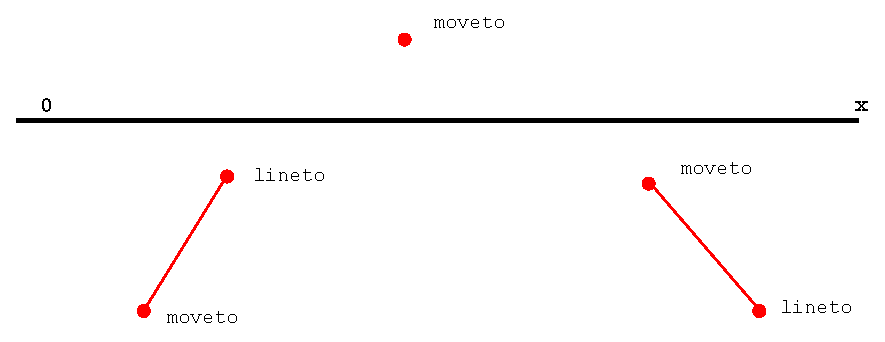
\includegraphics[width=1\linewidth]{ocasek-ilustrace.eps}
\caption{Ilustrace způsobu vykreslování grafu}
\end{figure}

%Důkladný popis programu pro jeho uživatele. Postup přeložení a sestavení programu na různých platformách (pokud se liší), popis ovládání všech funkcí programu a popis formátu datových souborů (pokud jsou a pokud jejich formát není zřejmý). Měla by být doplněna screenshoty nebo jinými vhodnými obrázky.
\section{Uživatelská příručka}
\label{sec:uziv_pr}
\subsection{Sestavení programu}
Program používá pouze standardní knihovny jazyka C. Při sestavování tedy není nutné linkovat platformě-specifické knihovny. Program je možné zkompilovat a slinkovat ručně, použitím vlastního kompilátoru, nebo využít připravených makefile. Při ruční kompilaci může být potřeba linkovat knihovnu math parametrem linkeru \emph{$-$lm}.
 
\subsubsection{Sestavení pomocí makefile}
Pro sestavení progrmau jsou připraveny dva soubory makefile.  

První (jméno \emph{makefile}) kompiluje překladačem gcc a pro odstranění souborů s objektovým kódem používá příkaz \emph{rm $-$rf}. Tento makefile je tedy určen spíš pro linuxové distribuce (testováno na distribuci Debian Wheezy 7.7).

Druhý (jméno \emph{makefile.win}) kompiluje překladačem cl (překladač od Microsoftu) a pro odstranění souborů s objektovým kódem používá příkaz \emph{del}. Z názvu vyplývá, že tento makefile je určen především pro Windows (testováno na Windows 7 64-bit). 

Výsledkem sestavení pomocí obou makefile je spustitelná aplikace graph.exe.

\subsection{Použití programu}
Program se spouští příkazem \emph{graph.exe $<$funkce$>$ $<$vystupni-soubor$>$ [$<$omezeni$>$]}. Paramery \emph{funkce} a \emph{vystupni-soubor} jsou povinné, parametr \emph{omezeni} je nepoviný, musí však dodržet níže popsaný formát.

Zápis matematické funkce musí být jednoznačný a nesmí být vynechán operátor násobení (místo 2x tedy 2*x). Názvy matematických funkcí a operátorů, které je možno použít, se nachází v kompletním zadání v sekci \nameref{sec:zadani}. K těmto funkcím jsou navíc přidány funkce \emph{cotan()} a \emph{acotan()}. 

Zápis funkce je umožněn s uvozovkami - "$x^2 + 1$" i bez nich. Při zadávání funkce bez uvozovek je však nutné vynechat všechny mezery - příkazový procesor by jinak funkci přečetl jako více argumentů a program by skončil chybou.

Parametr \emph{vystupni-soubor} je jméno výstupního souboru. Pokud bude uvedeno bez přípony, bude soubor bez přípony vytvořen. 

%shrnutí dosažených výsledků (např. časů běhu), zhodnocení splnění zadání, naznačení možných a žádoucích vylepšní, stručné shrnutí problémů, které se v semestrální práci vyskytly.
\section{Závěr}
%problémy s cl a definicí velikosti pole
%problémy se strncpy()
%chyba (-1)^2.5

\end{document}
